\chapter{Descripción y exploración de los datos}
\label{datos}


En este capítulo se describen las características principales de las series temporales hidro-climáticas utilizadas 
tanto para entrenar los modelos descritos en el capítulo \ref{ANNs}, 
como para ejecutar el modelo hidrológico MELCA y así generar las variables objetivos, es decir los caudales de descarga
 de las subcuencas.

\section{Series de precipitación}

La cuenca CHRC  posee una gran variación en la precipitación en un área geográfica reducida,
por este motivo los valores de precipitación recogidos por pluviómetros en las estaciones meteorológicas 
no son fácilmente extrapolables. Por otro lado los pluviómetros se encuentran 
a altitudes que se encuentran entre los 2000 y 3000 metros sobre el nivel del mar, mientras que el punto más alto de 
la cuenca se encuentra a  6288 m.s.n.m, lo que da lugar a que haya una deficiencia de datos en ciertos puntos geográficos. 
Para completar los datos en estos puntos se ha recurrido a las base de datos de ERA5 \cite{ERA5} y CHELSA \cite{CHELSA}.

Con el fin de contrastar si las series así obtenidas reflejan 
correctamente las variaciones del patrón de lluvias con la altura y la pendiente, 
se han analizado diversas bases de datos globales de precipitación, pero el resultado no ha sido 
satisfactorio.  Por ello, se ha optado por generar las series de manera sintéticas basándose 
en los patrones combinados de los pluviómetros y de las estaciones de aforos.



% Los datos de clima (precipitación y temperatura) fueron medidos a través de estaciones meteorológicas distribuidas de manera 
% irregular a lo largo de la cuenca. Las series disponibles reflejan adecuadamente las condiciones climáticas de las zonas 
% bajas y más pobladas, pero la información en las zonas más altas es escasa. 
% Los pluviómetros se encuentran a altitudes de entre los 2000 y 3000 metros sobre el nivel del mar, 
% mientras que el punto más alto de la cuenca se encuentra a las 6288 m.s.n.m

% Con el fin de contrastar si estas series reflejan 
% correctamente las variaciones del patrón de lluvias con la altura y la pendiente, 
% se han analizado diversas bases de datos globales de precipitación pero el resultado no ha sido 
% satisfactorio.  Por ello, se ha optado por generar las series de precipitación de manera sintéticas basándose 
% en los patrones combinados de los pluviómetros y de las estaciones de aforos.

% La cuenca del río Chambo posee una gran variación en la precipitación en un área geográfica reducida,
% por este motivo los valores de precipitación recogidos por pluviómetros en las estaciones meteorológicas 
% pueden no ser válidos para puntos lejanos. Es por eso que los datos correspondientes a puntos intermedios se 
% completaron a partir de la base de datos de ERA5 y CHELSA.

% \begin{figure}[h!]
%   \begin{center}
%     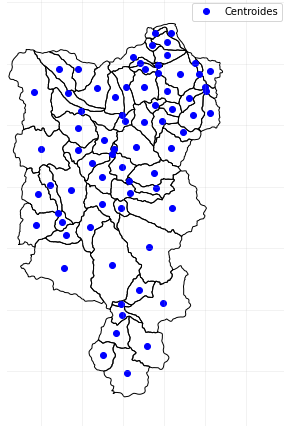
\includegraphics[height=3.in]{Figures/centroides.png}
%     \caption{ Localización de los centroides de las subcuencas}
%     \label{0}
%   \end{center}
% \end{figure}

%  Una vez que los huecos han sido rellenados, se han interpolado los datos recogidos por los pluviómetros a los centroides 
%  de las regiones  representadas en la figura \ref{0}. Este proceso consta de dos pasos, primero se estima si en un punto 
%  determinado va a llover (estimación kriging con la librería \textit{Krige} de r) y luego se estima la magnitud de dicha 
%  lluvia (Herrera et al., 2012).

%  \begin{figure}[h!]
%   \begin{center}
%     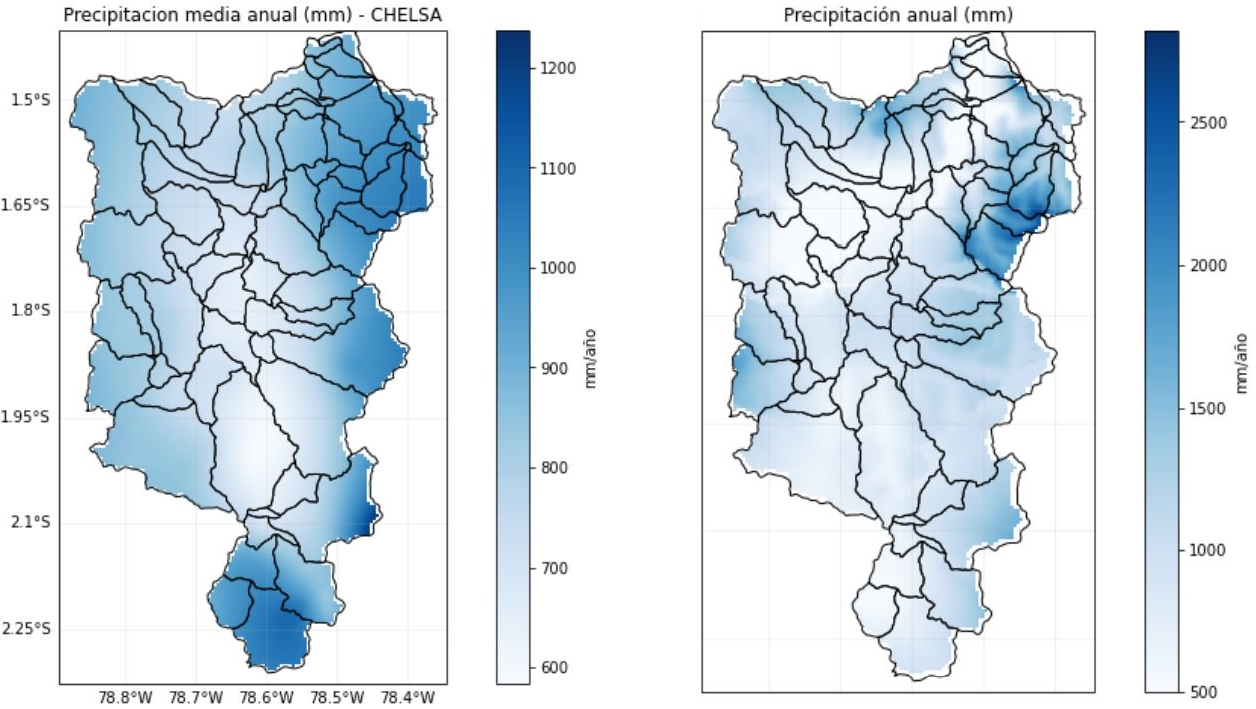
\includegraphics[height=3.in]{Figures/CHELSA_ERA5.jpg}
%     \caption{ Precipitación media anual (mm/año) basada en CHELSA (panel izquierdo) y en ERA5 (panel derecho).}
%     \label{1}
%   \end{center}
% \end{figure}


%  En la figura \ref{1} se muestra a modo de ejemplo los  valores de la precipitación media anual  obtenidos mediante interpolación 
%  sobre una malla regular de 100 m de lado utilizando la base de datos de ERA5 (panel derecho) y la de CHELSA (panel izquierdo).
%  Si bien los resultados reflejan correctamente la fuerte variabilidad de la precipitación en un area reducida, los patrones estacionales
%  así obtenidos no coinciden con los caudales y el conocimiento local. Es por eso que se ha optado por generar las series 
%  de manera sintética como se describe en la siguiente sección.



El modelo que genera las series de precipitación sintéticas diarias consta de dos niveles, 
primero se generan series mensuales y luego se generan series diarias desagregando los valores mensuales.
Para generar las series mensuales se parte del valor medio anual (determinado mediante en la interpolación de los 
datos de los pluviómetros con la base de datos CHELSA) en la región de interés y del valor medio en el 
mes más húmero. El modelo de desagregación a escala mensual asume que las precipitaciones acumuladas en cada mes 
siguen un comportamiento que puede ser representado por la siguiente distribución "Log-normal" 
que posee una variación temporal sinusoidal y desviación estándar $s_1$:

\begin{equation}
    P_m=exp\Bigg(N\bigg(a+b1\cdot cos\bigg(\frac{t-\phi_1}{6}\bigg)+b2\cdot cos\bigg(\frac{t-\phi_2}{12}\bigg)\bigg)\Bigg)
\end{equation}

$N(\mu,\sigma)$ es a su vez una distribución Gaussiana con media $\mu$ y desviación estándar $\sigma$. 
Los valores de las constantes $a$, $b_1$ y $b_2$ se obtienen a partir de la precipitación media y máxima, 
mientras que las fases $\phi_i$ dependen del régimen de precipitación.

% \begin{figure}[h!]
%     \begin{center}
%       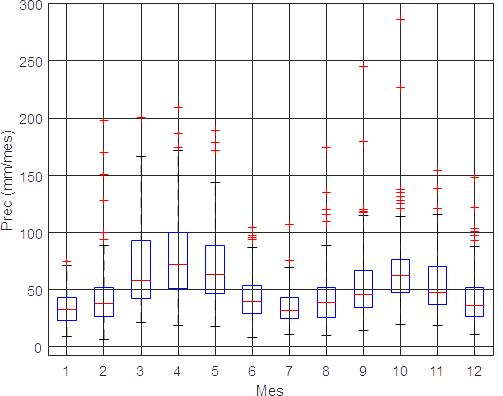
\includegraphics[height=3.in]{Figures/prec_sim.png}
%       \caption{ Valores simulados de precipitaciones mensuales en la zona de Guaslán}
%       \label{2}
%     \end{center}
%   \end{figure}


% En la figura \ref{2} se muestra a modo de ejemplo una de las series generada para una cuenca con clima costero, representativa del sector más 
% seco de la cuenca en la estación de Guaslán (cantón Riobamba). La línea roja representa el valor medio, la caja azul representa los valores situados entre los percentiles
%  25$\%$ y 75$\%$, y las barras negras los extremos (los puntos en rojo son tratados como datos atípicos). A modo de comparación,
%  en la figura \ref{3} se muestran los valores observados en la misma estación.

%  \begin{figure}[h!]
%     \begin{center}
%       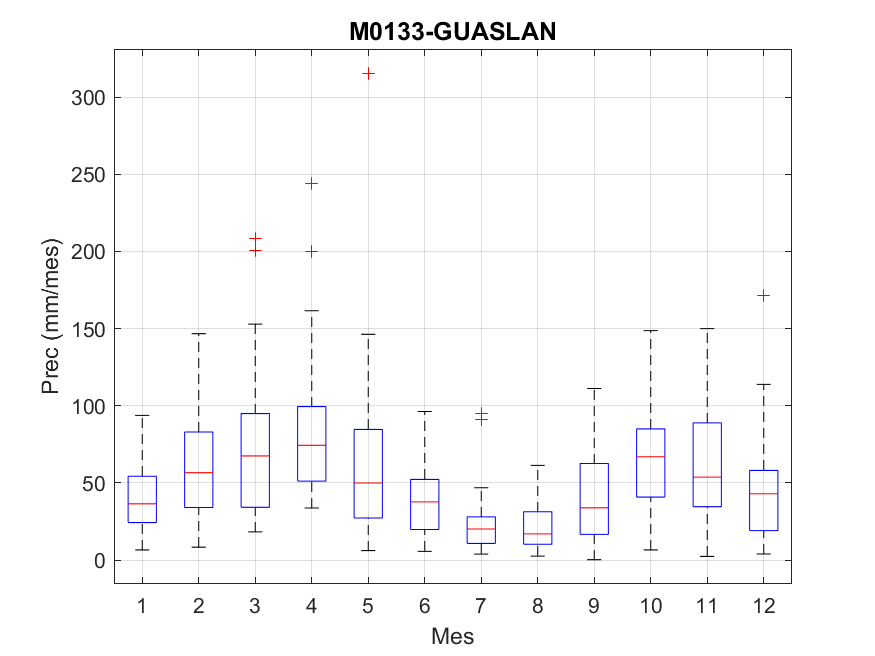
\includegraphics[height=3.in]{Figures/prec_obs.png}
%       \caption{ Valores observados de precipitaciones mensuales en la zona de Guaslán}
%       \label{3}
%     \end{center}
%   \end{figure}

%   \begin{figure}[h!]
%     \begin{center}
%       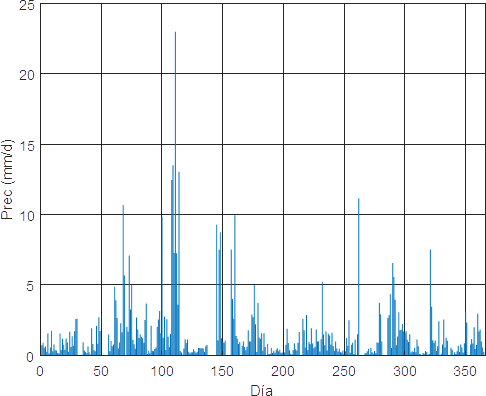
\includegraphics[height=3.in]{Figures/prec_sint.png}
%       \caption{ Un año de valores de precipitación diaria simulada en la zona de Guaslán}
%       \label{3}
%     \end{center}
%   \end{figure}


El modelo para crear las series diarias usa el método de cascadas aleatorias multiplicativas \cite{Molnar} para 
desagregar las series mensuales y posee dos parámetros: denominados $\sigma_2$ y $\beta$
que determinan la variabilidad e intermitencia de la lluvia (proporción media de días sin lluvia) y se usan para 
ajustar el modelo con los valores observados en las series de precipitación disponibles.


% \subsubsection{Comportamiento del régimen de precipitación}
% \label{regimenes_prec}
% Con el fin de poder realizar un estudio completo de cómo es el comportamiento del régimen de precipitaciones, 
% se seleccionaron 35 estaciones  meteorológicas que abarcan de manera uniforme el area de la cuenca de Chambo y sus alrededores.
% Se han identificado principalmente dos regímenes diferentes, un régimen bimodal en el oeste (dos períodos secos y dos de lluvias al año) 
% y el régimen monomodal (un período seco y uno de lluvias) en el este, con una franja que contiene un régimen mixto en 
% las zonas centrales de la cuenca.


\section{Series de temperatura}
\label{tempint}
Para la generación de las series de temperatura se han utilizado datos de 10 termómetros situados en el entorno del área de 
estudio.
Estos datos han sido sometidos a un proceso de curado que por un lado define una frontera para detectar outliers o datos
 atípicos siguiendo el siguiente criterio:
\begin{equation}
  si~X_i>5\cdot\sigma^2_n~es~un~utlier,~donde~\sigma^2_n=\frac{1}{n}\cdot\sum^n_{i=1}\bigg(X_i-\bar{X}\bigg)^2
\end{equation}
y por el otro lado elimina los datos que presentan un cierto grado de persistencia \cite{Estevez}
Los datos faltantes se han completado de manera similar a cómo se procedió con las series 
de precipitación utilizando los datos de ERA5.


\begin{figure}[h!]
  \begin{center}
    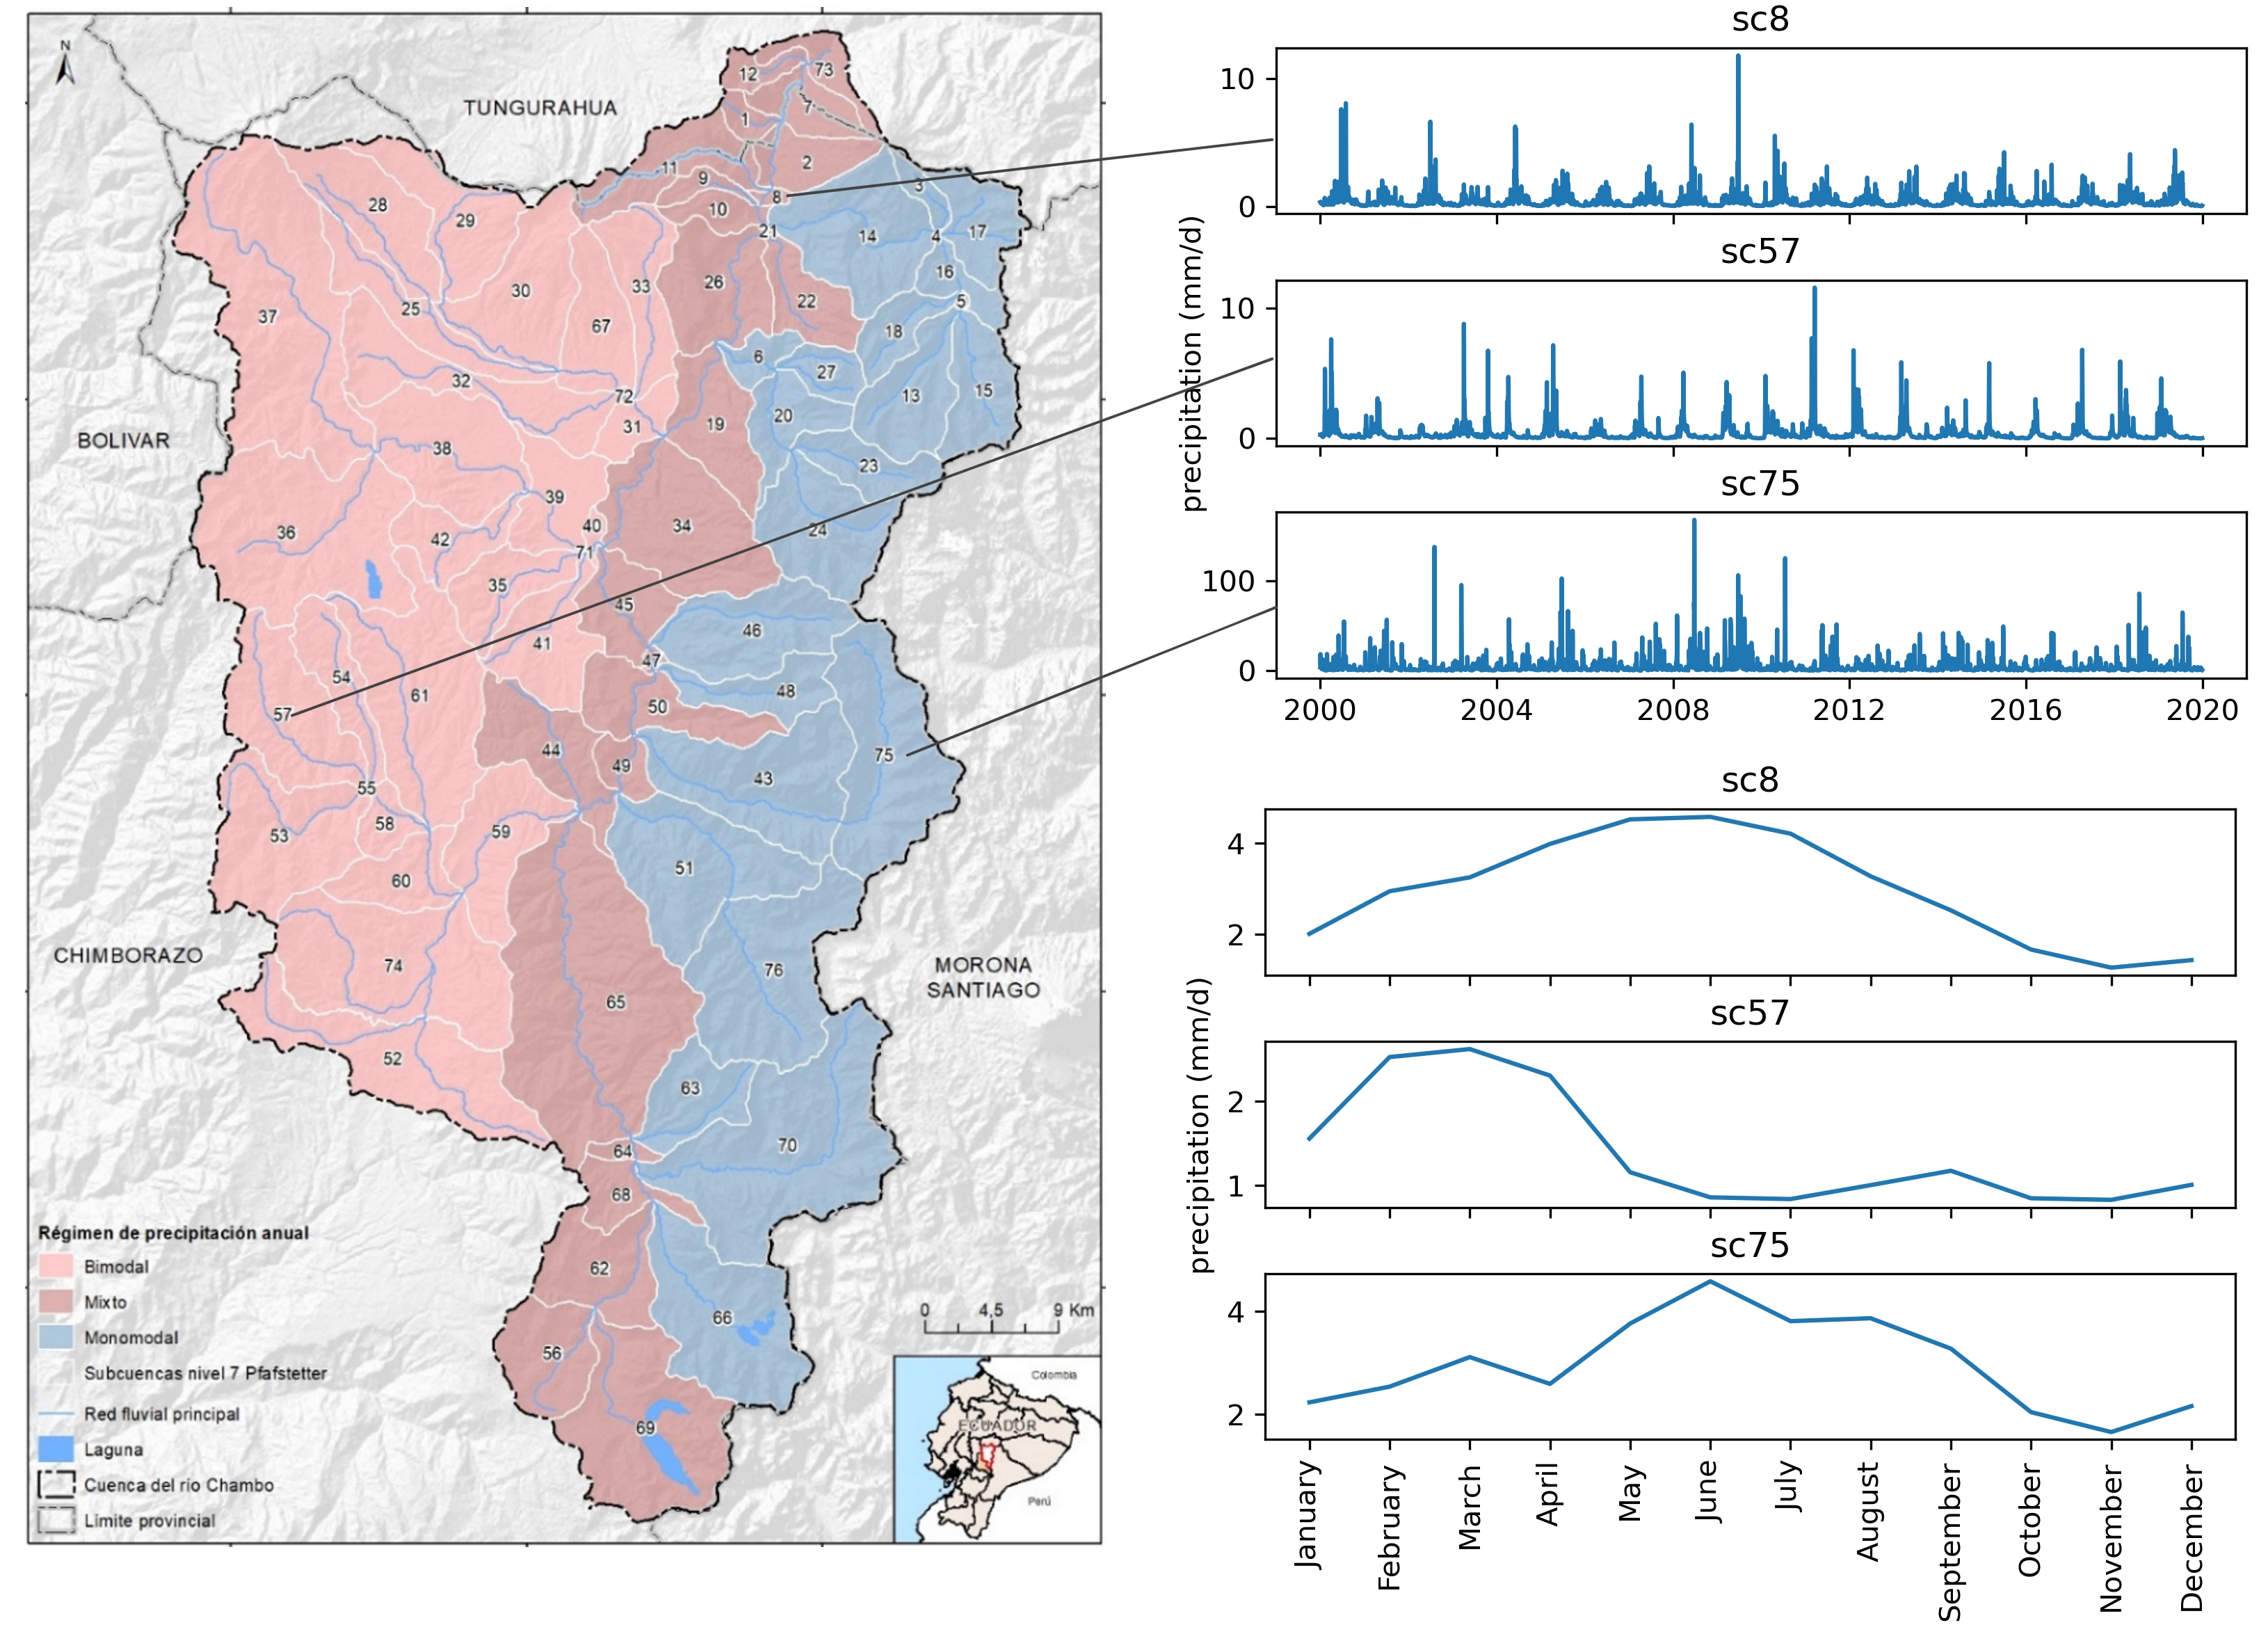
\includegraphics[height=6.5in]{Figures/cuenca_con_subcuencas_prec.png}
    \caption{ Series de precipitación para diferentes regiones de la cuenca Chambo. En los paneles superiores  
    se muestra la serie de precipitación correspondiente al año 2019 y  los valores medios mensuales desde el año 2000 hasta 
    el año 2020. En el panel inferior, se muestran las series de temperatura máxima y mínima diarias.}
    \label{4}
  \end{center}
\end{figure}

En la figura \ref{4}, se muestran a modo de ejemplo las series de precipitación y temperaturas
mínimas y máximas generadas para tres diferentes subcuencas 
localizadas en diferentes puntos de CHRC. Se pueden observar diferentes estacionalidades,
la cuenca con id = 57 presenta un  un régimen costero (donde la precipitación máxima tiene lugar entre Marzo-Abril), 
mientras que las cuencas con ids= 8 y 75, un régimen amazónico (con un único pico de precipitación en Junio-Julio).


